Este es es diagrama de secuencia de la llamada a la localizaci'on.
\begin{figure*}[h!]
	\begin{center}
        		\framebox{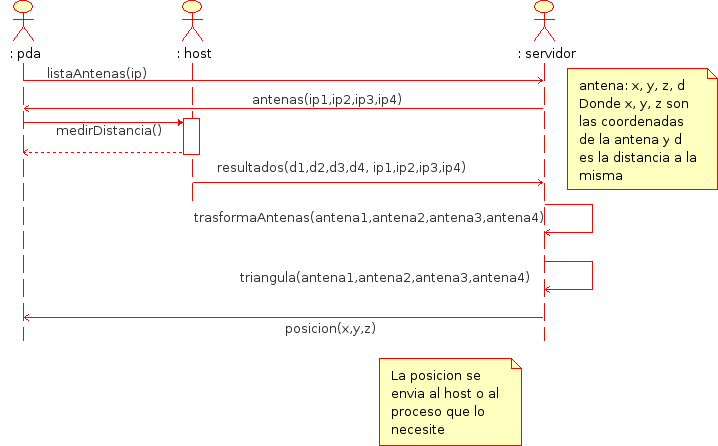
\includegraphics[scale=0.5]{localizador.png}}
     	\end{center}
    	\caption{Secuencia de localizaci'on}\label{fig:triang5}
\end{figure*}

La llamada a la funci'on triangula se encarga de la localizaci'on de la PDA una vez que se tienen medidas las distancias a los puntos de acceso.\bigskip \\ La localizaci'on corresponde a la resoluci'on del sistema de ecuaciones que se define por el punto de intersecci'on de tres esferas con centro el las coordenadas del punto de acceso y radio la distancia al dispositivo inal'ambrico a localizar. Si los puntos de acceso son:

\begin{enumerate}
\item Punto 1: 
	\begin{enumerate}
	\item Coordenadas: $(x_1,y_1,z_1)$
	\item Distancia: $d_1$
	\end{enumerate}

\item Punto 2: 
	\begin{enumerate}
	\item Coordenadas: $(x_2,y_2,z_2)$
	\item Distancia: $d_2$
	\end{enumerate}

\item Punto 3: 
	\begin{enumerate}
	\item Coordenadas: $(x_3,y_3,z_3)$
	\item Distancia: $d_3$
	\end{enumerate}

\item Punto 4: 
	\begin{enumerate}
	\item Coordenadas: $(x_4,y_4,z_4)$
	\item Distancia: $d_4$
	\end{enumerate}
\end{enumerate}

Para localizar el punto ($x$,$y$,$z$) tenemos que resolver:
\begin{enumerate}
	\item ecuación 1: $(x - x_1)² + (y - y_1)² +(z - z_1)² = d_1² $
	\item ecuación 2: $(x - x_2)² + (y - y_2)² +(z - z_2)² = d_2² $
	\item ecuación 1: $(x - x_3)² + (y - y_3)² +(z - z_3)² = d_3² $
	\item ecuación 1: $(x - x_4)² + (y - y_4)² +(z - z_4)² = d_4² $
\end{enumerate}

El cuarto punto lo usaremos para comprobar la correci'on de la resolucion o para reemplazar a uno de los anteriores si est'an alineados. En otro caso no es necesario porque sabemos que el punto a localizar est'a dentro del edificio.\bigskip\newline

La resoluci'on anal'itica directa genera denominadores del tipo $x_1 - x_2$, esos denominadores se anulan cuando las antenas est'an en las esquinas de un cuadrado. Esa situaci'on es frecuente asi que es necesario realizar una serie de translaciones y rotaciones para garantizar que los denominadores no se anulan. Hacemos que el origen del sistema de coordenadas est'e en el punto 1, el eje OX pase por el punto 2 y el plano XY pase por el punto 3. \bigskip\newline

\begin{figure*}[h!]
	\begin{center}
        		\framebox{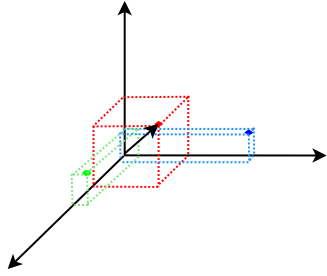
\includegraphics[scale=0.5]{Triangular1.png}}
     	\end{center}
    	\caption{Distribuci'on incial de los puntos}\label{fig:triang1}
\end{figure*}


El primer paso es transladar el origen al punto 1 $(x_1,y_1,z_1)$ desde el origen $(0,0,0)$. El vector de translaci'on es $V = (v_1,v_2,v_3) = (x_1,y_1,z_1) - (0, 0, 0)$. Aplicamos la rotaci'on a los tres puntos. 

\begin{figure*}[h!]
	\begin{center}
        		\framebox{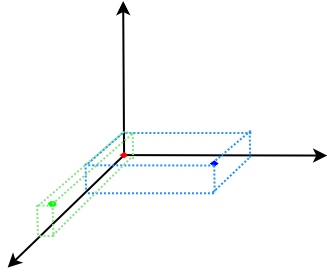
\includegraphics[scale=0.5]{Triangular2.png}}
     	\end{center}
    	\caption{Distribuci'on de los puntos tras la translaci'on}\label{fig:triang2}
\end{figure*}

Rotamos los ejes para transladar el eje OX y que pase por el punto 2.

\begin{figure*}[h!]
	\begin{center}
        		\framebox{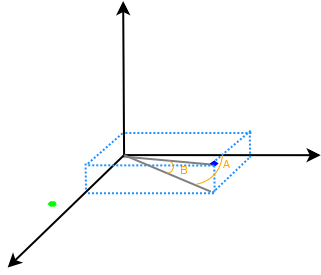
\includegraphics[scale=0.5]{Triangular3.png}}
     	\end{center}
    	\caption{'Angulos de rotaci'on}\label{fig:triang3}
\end{figure*}

Es necesario realizar dos rotaciones. La primera rotaci'on se corresponde al 'angulo a: $a = \arccos {x_2 \over {\sqrt{x_2²+z_2^2}}}$. El eje OX se alinea con la proyecci'on del punto 2 sobre el plano XZ. La nuevas coordendas del punto 2 son:

\begin{enumerate}
\item $x_2' = x_2 \sen a + z_2 \cos a$
\item $z_2' = - x_2 \sen a + z_2 \cos a$
\end{enumerate}

La segunda rotaci'on se corresponde al 'angulo b: $b = \arccos {x_2 \over {\sqrt{x_2²+y_2^2}}}$. El eje OX se alinea con el punto 2. La nuevas coordendas del punto 2 son:

\begin{enumerate}
\item $x_2' = x_2 \sen b + y_2 \cos b$
\item $y_2' = - x_2 \sen b + y_2 \cos b$
\end{enumerate}

Las rotaciones tambi'en afectan a los puntos 1 y 2. En el caso del punto 1 no es necesario realizar ninguna operaci'on pues se corresponde al origen. Los resultados para el punto 3 son análogos. \bigskip\newline

Rotamos los ejes para que el plano XY y que pase por el punto 3.

\begin{figure*}[h!]
	\begin{center}
        		\framebox{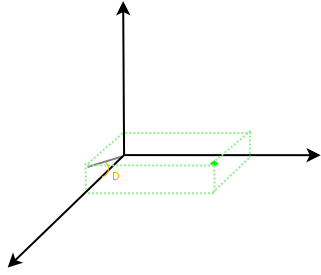
\includegraphics[scale=0.5]{Triangular5.png}}
     	\end{center}
    	\caption{'Angulos de rotaci'on}\label{fig:triang5}
\end{figure*}

La rotaci'on se corresponde al 'angulo d: $d = \arccos {y_3 \over {\sqrt{z_3²+y_3^2}}}$. El plano XY se alinea con la proyecci'on del punto 3 sobre el plano YZ. 

Tras la reosluci'on anal'itica es necesario dehacer estas modificaciones. 

\begin{enumerate}
\item Dehacemos la tercera rotaci'on -d grados.
\item Dehacemos la segunda rotaci'on -b grados.
\item Dehacemos la primera rotaci'on -a grados.
\item Transladamos -V.
\end{enumerate}

